%!TEX root = main.tex
\section{Grundlegendes}
\label{sec:defs}
    Zunächst wird ein Überblick über die nötigen Definitionen gegeben. Zuvor noch eine Beschränkung der Räume die in dieser Arbeit behandelt werden:


    \subsection{Die betrachteten Räume}
        Im Folgenden sei $M$ eine kompakte, orientierbare, zusammenhängende $3$-dimensionale Mannigfaltigkeit. Falls diese einen Rand hat, ist er homöomorph zu einer disjunkten Vereinigung von Tori.

        \todo{Hier rein über Glattheit <-> simpliziale approx wie in lee paul neuwirth}
        Um die Hilfsmittel zu erweitern oder Extremfälle auszuschließen, arbeitet man häufig in der Kategorie der stückweise linearen (PL, \textit{piecewise linear}) oder der differenzierbaren Mannigfaltigkeiten. Sieht man sich beispielsweise Knoten an, also Einbettungen $S^1 \into S^3$, so stellt man fest, dass diese besonders entartet aussehen können, allerdings nicht, falls es sich bei der Einbettung um eine PL oder differenzierbare Einbettung handelt. Ähnlich kann man in diesen Kategorien raumfüllende Kurven vermeiden. Allerdings stellte sich im Studium der $3$-Mannigfaltigkeiten heraus, dass die Situation sich erheblich von höheren Dimensionen unterscheidet, beispielsweise ist nicht jede Gruppe als Fundamentalgruppe einer $3$-Mannigfaltigkeit realisierbar \todo{ref(später)}. Außerdem lässt es sich ergiebig ausnutzen, dass in Dimension $3$ keine Unterscheidung der topologischen, PL und differenzierbaren Mannigfaltigkeiten übereinstimmen: nach Moise's Theorem besitzt jede $3$-Mannigfaltigkeit sowohl eine eindeutige PL als auch eine eindeutige differenzierbare Struktur. Das bedeutet, um Aussagen für $3$-Mannigfaltigkeiten zu zeigen, kann man sich (fast) beliebig in diesen Kategorien hin- und herbewegen um das Resultat am Ende für alle zu erhalten. Um diese beiden Beispiele hervorzuheben, lässt sich bemerken, dass für $4$-Mannigfaltigkeiten überabzählbar viele unterschiedliche differenzierbare Strukturen besitzen und auch jede Gruppe, Fundamentalgruppe einer $4$-Mannigfaltigkeit ist.\\
        Diese Arbeit wird sich jedoch konsistent in der $C^\infty$ Kategorie bewegen. Der vorherige Abschnitt dient also lediglich der Betonung, dass dies keine Einschränkung bedeutet. 


    \subsection{Alexander Invarianten}
    	Ein Clou der folgenden Methoden ist es, die Struktur einer Überlagerung --- genauer gesagt ihre Decktransformationen --- auszunutzen, indem man den Gruppenring betrachtet. Der Gruppenring $R[G]$ ist algebraischer Herkunft und kann für allgemeine kommutative Ringe $R$ und Gruppen bzw. Monoide $G$ definiert werden, jedoch genügt es für diese Arbeit eine speziellere Definition heranzuziehen, für den Fall das $G=F$ eine endlich erzeugte freie abelsche Gruppe und $R=\ZZ$ ist.
    	\begin{defn}[Gruppenring]
    		Sei $F$ eine freie abelsche Gruppe. Dann ist der \textit{Gruppenring} definiert als:
    		\[
    			\ZZ[F] = \sum_{i \in I} a_i f_i, a_i \in \ZZ, f_i \in F, |I| < \infty
    		\]
    	\end{defn}
        \label{wirkung:gruppenring}
    	Falls also $F$ nun eine unendlich zyklische Gruppe mit Erzeuger $t$ ist, lässt sich der Gruppenring über $F$ als $\ZZ[F] = \ZZ[t^{\pm 1}]$, also als Ring der formalen Laurentpolynome in der Variablen $t$ auffassen. 
    	Grundlage für die Definitionen der Alexander Invarianten ist die zur Abelianisierung der Fundamentalgruppe gehörende Überlagerung. Allgemeiner sei $M$ eine 3-Mannigfaltigkeit mit den obigen Beschränkungen und $\phi: G=\pi_1(M) \to F$ ein Homomorphismus in eine freie abelsche Gruppe F. Aus der Überlagerungstheorie ist bekannt, dass nun eine zusammenhängende Mannigfaltigkeit $\hat M_\phi$ existiert, die $M$ überlagert und auf Level der Fundamentalgruppen $ker \phi \cong \pi_1 (\hat M_\phi) \stackrel{p_*}{\hookrightarrow} \pi_1(M)$ einbettet. Diese ist bis auf Homöomorphie eindeutig. Die Decktransformationsgruppe ist dann isomorph zum Quotienten $\pi_1(M)/p_*\pi_1(\hat M_\phi) \cong F$. Dieser operiert dann auf $\hat M_\phi$ durch Homöomorphismen, induziert also auch eine Operation auf $\pi_1(\hat M_\phi)$ und auf $H_1(\hat M_\phi)$. Da $\ZZ$ auf jeder abelschen Gruppe wirkt, ist folgende Definition gerechtfertigt:
    	\begin{defn}[Alexander Modul]
    		Der Alexander Modul ist definiert als
    		\[
    			A_\phi(M) = H_1(\hat M_\phi)
    		\]
    		aufgefasst als $\ZZ[F]$-Modul, mit der induzierten Wirkung der Decktransformationen.
    	\end{defn}
    	Es wird sich bei weiterer Inspektion herausstellen, dass der Alexander Modul im Fall einer kompakten 3-Mannigfaltigkeit immer endlich erzeugt ist. 
    	Da es sich bei dem Gruppenring nicht um einen Hauptidealring handelt, ist es im Allgemeinen nicht möglich eine Zerlegung des Alexander Moduls in zyklische direkte Summanden zu finden. Als algebraische Invariante, wird dem Modul stattdessen hier ein Reihe von Idealen in dem Gruppenring zugewiesen --- die Elementarideale. Da der Alexander Modul endlich erzeugt über dem Gruppenring ist, existiert eine freie Auflösung, aus derer Präsentation für den Modul wir die Elementarideale gewinnen möchten. Betrachte die endliche Präsentation:
    	\[
    		\ZZ[F]^k \stackrel{X}{\to} \ZZ[F]^n \stackrel{\alpha}{\to} A_\phi(M) \to 0
    	\]
    	wobei $X$ eine darstellende Matrix bezüglich der kanonischen Basen $e_1, \cdots , e_k$ und $e'_1, \cdots ,e'_n$ ist. Diese Präsentationsmatrix ist bis auf Vertauschen von Zeilen, Hinzufügen von Einheitsblöcken oder Nullspalten und Addieren eines Vielfachen einer Spalte oder Zeile auf eine jeweils andere eindeutig. Das liefert die nächste Definition
    	\begin{defn}
    		Definiere das $i$-te Elementarideal von $M$ bezüglich $\phi$ $E_i(A_\phi(M)) \subset \ZZ [F]$ als das von den $(n-i-1)$-Minoren erzeugte Ideal.  
    	\end{defn}

    	Natürlich lassen sich Elementarideale für alle endlich präsentierten Moduln über kommutativen Ringen analog definieren.

    	Falls $\phi$ die Abelianisierung ist, definiert diese Invariante des Alexander Moduls natürlich auch eine Invariante der Mannigfaltigkeit. Nun ist $\ZZ[F]$ kein Hauptidealring, jedoch ist es durchaus interessant als weitere Invariante das kleinste Hauptideal zu betrachten das ein Elementarideal enthält.
    	\begin{defn}(Alexander Polynom)
    		Definiere das Alexander Polynom $\Delta_\phi$ als einen größten gemeinsamen Teiler von $E_1(A_\phi(M))$.
    		%Ist das überhaupt definiert wenn phi nicht Abelianisierung?
    	\end{defn}
    	\begin{bem}
    		In dem Gruppenring sind die Einheiten genau die Gruppenelemente. (im Allgemeinen nicht ganz). Das Alexander Polynom ist also bis auf Multiplikation mit einem Gruppenelement aus dem Gruppenring wohldefiniert.
    	\end{bem}

    	Bleibt nur noch die Alexander Norm zu definieren, die eine Norm auf der ersten Kohomologie der 3-Mannigfaltigkeit beschreibt.
    	\begin{defn}
    		Sei  $\Delta \in \ZZ [F]$ das Alexander Polynom das zu der Abelianisierung der Fundamentalgruppe gehört. So ist $\Delta$ von der Form:
    		\begin{align*}
    		    			\Delta = &\sum_{k=1}^n a_k f_k& a_k \neq 0, f_i = f_j \Rightarrow i=j
    		\end{align*}
    		Sei nun $\phi \in \Hom (F,\ZZ) \cong H^1 (M,\ZZ)$, dann definieren wir die Alexander Norm von $\phi$ als
    		\[
    			||\phi||_A = \begin{cases}
    				0 , &\text{ wenn } \Delta=0\\
    				\sup \phi (f_i - f_j) &
    			\end{cases}
    		\]
    		Wobei das Supremum über die Gruppenelemente $f_i$ genommen wird, die in $\Delta$ auftauchen.

    	\end{defn}

    \subsection{Thurston Invariante}
        Ziel ist es eine weitere Norm auf der ersten Kohomologie der kompakten 3-Mannigfaltigkeit zu definieren. Poincaré Dualität liefert in diesem Fall einen Isomorphismus $H^1(M;\ZZ) \to H_2(M;\ZZ)$. Eine zu $\phi \in H^1(M,\ZZ)$ duale Fläche wird später noch explizit beschrieben werden. Tatsächlich ist es sogar ein bedeutendes Zwischenresultat, das eine solche Fläche immer mit Eigenschaften gewählt werden kann die bestimmten Abschätzungen genügen. Auf der anderen Seite sollte so eine gewählte Fläche auch eine Minimalitätseigenschaft erfüllen und zwar bezüglich der folgenden Norm:
        \begin{defn}[Thurston Norm]
        	Definiere die Thurston Norm für $\phi \in H^1(M,\ZZ)$ als
        	\[
        	        		||\phi||_T = \{\min \chi_-(S)| \text{ S ist orientierbar eingebettete Fläche dual zu } \phi \},
        	        	\]        	
        	wobei $\chi_-(S)=\sum \max (-\chi(S_i),0)$  und $S=\sqcup S_i$ die Zusammenhangskomponenten von $S$ sind.
        \end{defn}


        Als Abschluss dieses einführenden Kapitels, soll noch folgendes essentielles --- wenn auch im Folgenden nicht zwingend benötigtes --- Lemma gezeigt werde:
        \begin{lem}
        \label{lem:norm}
        	Die Alexander Norm und die Thurston Norm definieren Halbnormen auf der ersten Kohomologie einer kompakten 3-Mannigfaltigkeit. 
        \end{lem}
        \newpage blabla\\
          \noindent\textit{Beweis.}
            Bei der Alexander Norm ist nichts zu zeigen, die Halbnormeigenschaften ergeben sich unmittelbar aus der Definition.\\
            Im Falle der Thurston Norm, ist das Lemma Gegenstand der ersten zwei Kapitel aus \cite{Thurston1986}, dessen Beweis mit leichten Anpassungen im Folgenden kurz skizziert werden soll.
            Es muss die Skalarmultiplikativität und die Subadditivität gezeigt werden also:
            \begin{align}
                ||\lambda\phi||_T & = \lambda ||\phi||_T ,&\lambda \in\ZZ \label{eq:scalarmul} \\
                ||\phi + \psi||_T &\leq ||\phi||_T + ||\psi||_T ,& \phi,\psi \in H^1(M) \label{eq:subadd}
            \end{align} 


            Da die Thurston Norm aus den Eigenschaften der dualen Flächen hervorgeht, ist es nötig sich Gedanken zu den Homologieklassen zu machen. Dann ist für \ref{eq:scalarmul} offensichtlich ein gutes Indiz, falls für repräsentierende, orientierte, eingebettete Flächen, dessen Homologieklassen sich teilen, also $S,T$ mit $[S],[T]\in H_2(M,\partial M)$ und $[S]=\lambda [T]$, das Vielfache $S$ bereits disjunkte Vereinigung von $\lambda$ zusammenhängenden Komponenten $S_i$ ist, mit $[S_i]=[T]$. \\
            Für $[S]=\phi \in H^1(M;\ZZ)$, existiert eine glatte Abbildung $f:M \to S^1$ die $\phi$ repräsentiert, in obigem Sinne. Urbilder regulärer Werte ergeben nach \todo{regwert} duale Flächen. Nun geht aus der später Folgenden Konstruktion~\ref{constr:presurf} hervor, dass ohne Einschränkung $S=f^{-1}(s)$ gewählt werden kann, also dass jede Fläche so repräsentiert werden kann. Sei deswegen auch $g:M \to S^1$ glatt mit dem regulären Wert $t$, sodass $g^{-1}(t)=T$. Betrachtet man die Überlagerung $p: S^1 \stackrel {z^\lambda} \to  S^1$, liefert wegen $\im\pi_1(f) \subset \lambda \ZZ$, die Überlagerungstheorie einen eindeutigen Lift $\hat f$:
            \[
                \begin{xy}
                    \xymatrix{M \ar[r]^{\hat f} \ar[d]_g \ar[dr]^f&S^1 \ar[d]^p \\
                             S^1 \ar[r]_p & S^1}
                \end{xy}
            \]
            Das Quadrat kommutiert bis auf Homotopie, also $p\hat f \simeq p g$, denn beide Abbildungen identifizieren sich unter der Bijektion $H^1(M;\ZZ) \cong [M,S^1]$ mit $\lambda \phi$, also impliziert die Existenz dieser Bijektion, dass $[p\hat f] = [pg]$. Somit folgt auch, dass Urbilder regulärer Werte aus $S^1$ unter $\hat f$ homolog zu solchen aus $g$ sind. Da $p^{-1}(s)=\{s_1,\cdots,s_n\}$ sicher reguläre Werte von $\hat f$ sind (folgt zum Beispiel aus der Kettenregel für Differentiale), sind die Urbilder $S_1,\cdots,S_n$ disjunkte, eingebettete, orientierte Flächen mit $[S_i]=[T]$. Da $S$ auch minimal (bezüglich der Thurston-Norm) gewählt werden kann, folgt also $||[S]||_T \geq \lambda ||\frac 1\lambda [S]||_T = \lambda ||T||_T$. Nun lässt sich aber aus einer minimierenden Fläche für $T$ (sei $T$ selbst so gewählt), zum Beispiel aus der zweiseitigen glatten Einbettung $T \times (-\epsilon,\epsilon) \to M$, $\lambda$ disjunkt eingebettete Kopien von $T$ gewinnen, die selbstverständlich auch $[S]$ repräsentieren, also $||\lambda \phi||_T = \lambda ||\phi||_T$.\\

            Um nun die Subbadditivität \ref{eq:subadd} zu zeigen, ist es nötig sich die Geometrie der $||\cdot||_T$-minimierenden Flächen $S,T$ mit $[S]=\phi, [T]=\psi$ genauer zu betrachten. Die Differentialtopologie liefert mit dem Transversalitätstheorem diffeotope Approximationen von $T$, die transversal zu $S$ sind, deswegen seien also ohne Einschränkung $S \transversal T$ transversal (Es folgt außerdem durch die Transversalität, dass $S\cap T$ eine glatte, kompakte 1-Mannigfaltigkeit ist (Pullback bleibt in Kategorie). Die Klassifikation von 1-Mannigfaltigkeiten liefert, dass diese also eine disjunkte Vereinigung von Kreisen und abgeschlossenen Intervallen ist). Des Weiteren soll ohne Einschränkung keine Komponente des Schnittes $S\cap T$  eine Scheibe beranden, die in $S$ oder $T$ enthalten ist. Diese Annahme kann man wie folgt einsehen:\\
            \begin{wrapfigure}{r}{0.5\textwidth}
                \label{fig:surgery}
                \centering
                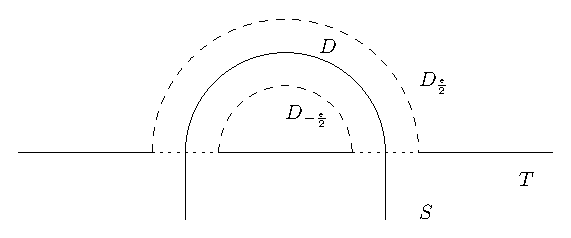
\includegraphics[width=0.49\textwidth]{surgery}
                \caption{Ausschneiden einer Umgebung von $S\cap T$ und Ankleben zweier Scheiben, sodass die Homologieklasse erhalten bleibt}
            \end{wrapfigure}
            Ohne Einschränkung sei die Scheibe $D$ mit einer solchen Komponente $\partial D \subset S \cap T$ als Rand, auf dem Inneren disjunkt von $T$, da sie ohne Einschränkung in $S$ liegt, und ein nichttrivialer Schnitt mit $T$ eine Komponente aus $S\cap T$ liefert, deren trivialer Nullbordismus in $S$ dank Transversalität, weniger Komponenten im Schnitt mit $T$ hat als die ursprüngliche Scheibe. So fahre man endlich oft fort, bis der Durchschnitt trivial ist beziehungsweise die berandete Scheibe, $T$ nicht berührt. Nun lässt sich eine hinreichend kleine offene Tubenumgebung von $\partial D$ aus $T$ entfernen. Diese kann wie folgt gewählt werden: sei $\nu(S) \to M$ eine Tubenumgebung von $S$ die sich aufgrund der Zweiseitigkeit wie folgt wählen lässt: $\alpha: S \times (-\epsilon,\epsilon) \to M$, sodass $\im\alpha|_{S\times (-\frac 12\epsilon,\frac 12 \epsilon)} \cap T$ eine Tubenumgebung von $S\cap T \subset T$ ist. Dann lässt sich diese Tubenumgebung bei $\partial D$ aus $T$ entfernen und mittels der Zweiseitigkeit um $D$, findet man zwei Kopien $D_{\frac \epsilon 2}, D_{-\frac \epsilon 2}$ sowieso Anklebevorschriften, mit denen diese Scheiben an die beiden durch Ausschneiden entstandenden Kreis-Randkomponenten kleben kann. Als Resultat ergeben sich Flächen $S,T'$, deren Durchschnitt um eine Komponente reduziert wurde und offensichtlich $[T]=[T']$ gilt. \todo{kein Weg aus dem Durchschnitt ist rel Endpunkt homotop zu einem Rand}\\
            Von nun an seien $S,T$ transversale Flächen, deren Durchschnitt den obigen Anforderungen genügt. Ziel ist es nun, den Zykel, der die Vereinigung repräsentiert, als eingebettete Fläche zu repräsentieren. Beachtet man die Orientierungen, so kann man an jeder Komponente des Durchschnitts die Vereinigung aufschneiden (die lokal aussieht wie die Gerade an der sich zwei orientierte Ebenen im $\RR^3$ schneiden), und entlang der Orientierungen in nur einer Möglichkeit wieder verkleben, so dass man eine Mannigfaltigkeit erhält (dies funktioniert offensichtlich an den Durchschnittkomponenten mit Rand, aber auch den den geschlossenen Komponenten, da die Orientierungen auf $S$ und $T$ global gewählt sind). Natürlich können alle diese Klebe- und Schneideprozesse glatt durchgeführt werden. Nun erhält man eine glatte, orientierte Fläche $U$, die (nach gegebenfalls leichter Modifikation) auch eigentlich eingebettet ist. Nun muss dieses Ergebnis und die Auswirkungen der Konstruktionen auf die Flächen diskutiert werden. Die uneinschränkenden Konstruktionen zu Beginn, können natürlich die Euler Charakteristik verändern, jedoch resultieren daraus weiterhin Thurston-Norm minimierende Flächen. Zwei solche Flächen gegeben, erbt die letztere Konstruktion, die aus $S\cup T$ eine homologe Fläche macht, die Summe der Eulercharakteristika:
            \begin{eqnarray*}
                \chi(U) = \chi(S) + \chi(T) &\implies& \chi_-(U)=\chi_-(S) + \chi_-(T) 
            \end{eqnarray*}
            , wobei die Implikation gilt, da bei der Konstruktion von $U$ keine Komponenten mit positiver Eulercharakterstik entstehen, unter den an $S$ und $T$ gestellten Annahmen. Dies liefert nun die Subbadditivität der Thurston-Norm auf den Homologieklassen.
        \qed

        Häufig stellt man Annahmen an die 3-Mannigfaltikeit, die es verbieten, dass Homologieklassen von Sphären oder Tori repräsentiert werden können. In dem Fall würde dann sogar $||\phi||_T=0 \Leftrightarrow \phi=0$ gelten. Dies alles motiviert natürlich, diese Norm zu einer Vektorraumnorm auf $H^1(M;\QQ)$ oder $H^1(M;\RR)$ fortzusetzen. 
        \begin{bem}[Fortsetzung von $||\cdot||_T$]
        \label{rem:extendingthurston}
            Will man $||\cdot||_T: H^1(M;\ZZ) \to \RR$ fortsetzen, so hilft die in Lemma~\ref{lem:norm} gezeigte Skalarmultiplikativität. Da $H^1(M;\ZZ)$ als $\ZZ$-Modul frei mit Rang $n$ ist, liefert die Einbettung $\ZZ^n \into \QQ^n$ zusammen mit der Linearität der Thurston-Norm eine lineare Fortsetzung auf den Strahlen (1-dimensionale Untervektorräume), die von Gitterpunkten erzeugt werden. Da aber für jedes $q \in \QQ^n$, bereits $aq \in \ZZ^n$ gilt (für großes $a\in \ZZ$), liefert dies bereits eine Fortsetzung auf $H^1(M;\QQ)$. Nun ist aber diese Fortsetzung eine konvexe Funktion, also auf jedem Kompaktum Lipschitz-stetig und somit auf jedem Kompaktum $K\cap \QQ^n, K\subset \RR^n$ in eindeutiger Weise stetig auf $K$ fortsetzbar --- es folgt die Existenz von $||\cdot||_T:H^1(M;\RR) \to \RR$.
        \end{bem}
        Nun stehen die Definitionen der Invarianten bereit, die auf den folgenden Seiten untersucht werden sollen.
